\documentclass[tikz,border=10pt]{standalone}
\usepackage{tikz}
\usetikzlibrary{angles,quotes,calc}
\usepackage{tkz-euclide} %for right angle marker

\begin{document}
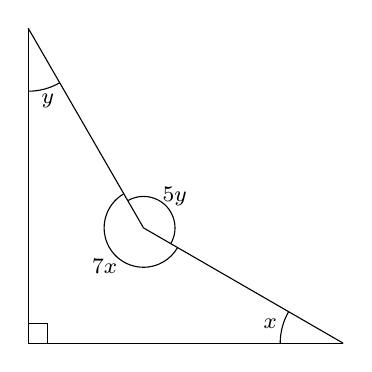
\begin{tikzpicture}[scale = 1]
    % Initial point
    \coordinate (A) at (0,0);
    % Draw base
    \draw (A) -- (4,0) coordinate (B);
    
    % Draw triangle
    \draw (A) -- ++(90:4cm) coordinate (C);
    \path[name path=leg2] (B) -- ++(180 - 30:3.5cm);
    \draw (A) -- (C);
    \path[name path = leg1] (C) -- ++(-90+30:3cm);
    
    \draw[name intersections={of=leg1 and leg2,by={Int1}}] (C) -- (Int1);
    \draw (Int1) -- (B);
    
    % Draw the angle between lines
    \pic [draw, "\footnotesize $x$ ", angle eccentricity=1.2, angle radius=0.8cm] {angle = Int1--B--A};
    \pic [draw, "\footnotesize $y$", angle eccentricity=1.2, angle radius=0.8cm] {angle = A--C--Int1};
    \pic [draw, "\footnotesize $7x$", angle eccentricity=1.4, angle radius=0.5cm] {angle = C--Int1--B};
    \pic [draw, "\footnotesize $5y$ ", angle eccentricity=1.4, angle radius=0.4cm] {angle = B--Int1--C};
    %marking right angles
    \tkzMarkRightAngle[size=.25](B,A,C);
   
\end{tikzpicture}
\end{document}

